\documentclass[12pt]{article}

\usepackage{fullpage}
\usepackage{multicol,multirow}
\usepackage{tabularx}
\usepackage{ulem}
\usepackage[utf8]{inputenc}
\usepackage[russian]{babel}
\usepackage{graphicx}
\usepackage{indentfirst}


\begin{document}

\section*{Лабораторная работа №\,1 по курсу дискрeтного анализа: сортировка за линейное время}

Выполнил студент группы М08-207Б МАИ \textit{Цапков Александр}.

\subsection*{Условие}

\begin{enumerate}
\item Требуется разработать программу, осуществляющую ввод пар «ключ-значение»,
 их упорядочивание по возрастанию ключа указанным алгоритмом сортировки за линейное
 время и вывод отсортированной последовательности.
\item Поразрядная сортировка.

Тип ключа: MD5-суммы (32-разрядные шестнадцатиричные числа).

Тип значения: строки фиксированной длины 64 символа, во входных данных могут встретиться строки меньшей длины, при этом строка дополняется до 64-х нулевыми символами, которые не выводятся на экран.

 
\end{enumerate}

\subsection*{Метод решения}

При решении задачи я использовал указанный в моем варианте алгоритм сортировки: поразрядная сортировка. Данный алгоритм представляет собой сортировку за линейное время и производится по средствам поразрядной сортировки начиная с наименьшего разряда другой устойчивой сортировкой: сортировкой подсчетом. При сортировки подсчетом создается массив в котором производится подсчет входных значений и который, в конце концов, начинает указывать на то место на которое нужно поставить изначальные вхождения. Таким образом мы можем отсортировать к примеру массив только по 1 разряду.  Сложность сортировки подсчетом О(n+k), где k -  это максимальное значение, а n - количество вхождений. При k многопривышающим n данный алгоритм наиболее эффективен именно это и происходит при поразрядной сортировки, где максимальное значение - это разряд системы (10-ичная 2-ичная и тп). Если известна изначально длинна вхождений, то для наибольшей эффективности можно посчитать «в какой системе» производить поразрядную сортировку (сколько бит за раз брать) $Log_2 (b)$.

\subsection*{Описание программы}

Так как в задаче мне нужно отсортировать вхождения ключ-значение, то я создал структуру $keyVal$ с фиксированным размером ключа и значения (так как по заданию они фиксированы).  Также я написал класс вектора TVector в файле Vector.hpp для динамического заполнения вхождений (нам не известно в начале количество вхождений). В функции $main$ мы заполняем структуру $keyVal$ из стандартного входа и копируем ее в наш вектор и повторяем этот процесс до конца входящих значений. Таким образом у нас получается заполненный вектор структур с ключами в виде строки чаров и значениями в виде строки чаров. После этого вызывается функция $RadixSort$, которая поразрядно вызывает функцию $CountingSortInDig$, сортировку подсчетом по данному разряду. Сортировка подсчетом выполняется на сомой строке, так как мы можем просто вызывать нужный разряд в массиве чаров через $key[i]$, где $i$ — это индекс разряда, а потом в маловесной функции $Atoi$ преобразововать чар в нужный нам $int$ (для 16-ричной цифры). Это эффективнее чем делать $div$ и $mod$, но менее эффективно чем побитовая сортировка, но поскольку преобразование этой строки в 128и битное значение тоже будет занимать какое-то лишнее время, я решил этим пренебречь. 

После выполнения всех этих операций мы получаем отсортированный вектор, который потом и выводим. Поскольку для ввода и вывода я использовал только функции c++, я отключил синхронизацию потоков, для более быстрого ввода вывода.

Источник: внимательно слушал Никиту Константиновича Макарова на лекциях.

\subsection*{Дневник отладки}

1-2 Попытки: настраивал $clean$ опцию в мэйкфайле для чекера. Полностью убрал все инструкции из clean.

3 Попытка: превышено время ожидания, добавил строку для отключения синхронизации потоков.

4 Попытка: случайно заменил >> на , в воде $cin$, что привело к бесконечному циклу.

5 Попытка: программа прошла все тесты, но я поправил Code Style.

\subsection*{Тест производительности}
Для проверки скорости программы и линейности алгоритма я немного модифицировал файл main, для того чтобы он сам создавал рандомные ключи и одинаковые value значения (так как мне нужно узнать только скорость алгоритма, а правильность его я уже проверил на тестах). Таким образом с измененным исходным кодом я ввожу число, которое означает количество вхождений и получаю время выполнения в миллисекундах. Полученные результаты можно видеть на графике, где по оси $x$ — отложено количество вхождений, а по оси $y$ — время в миллисекундах.

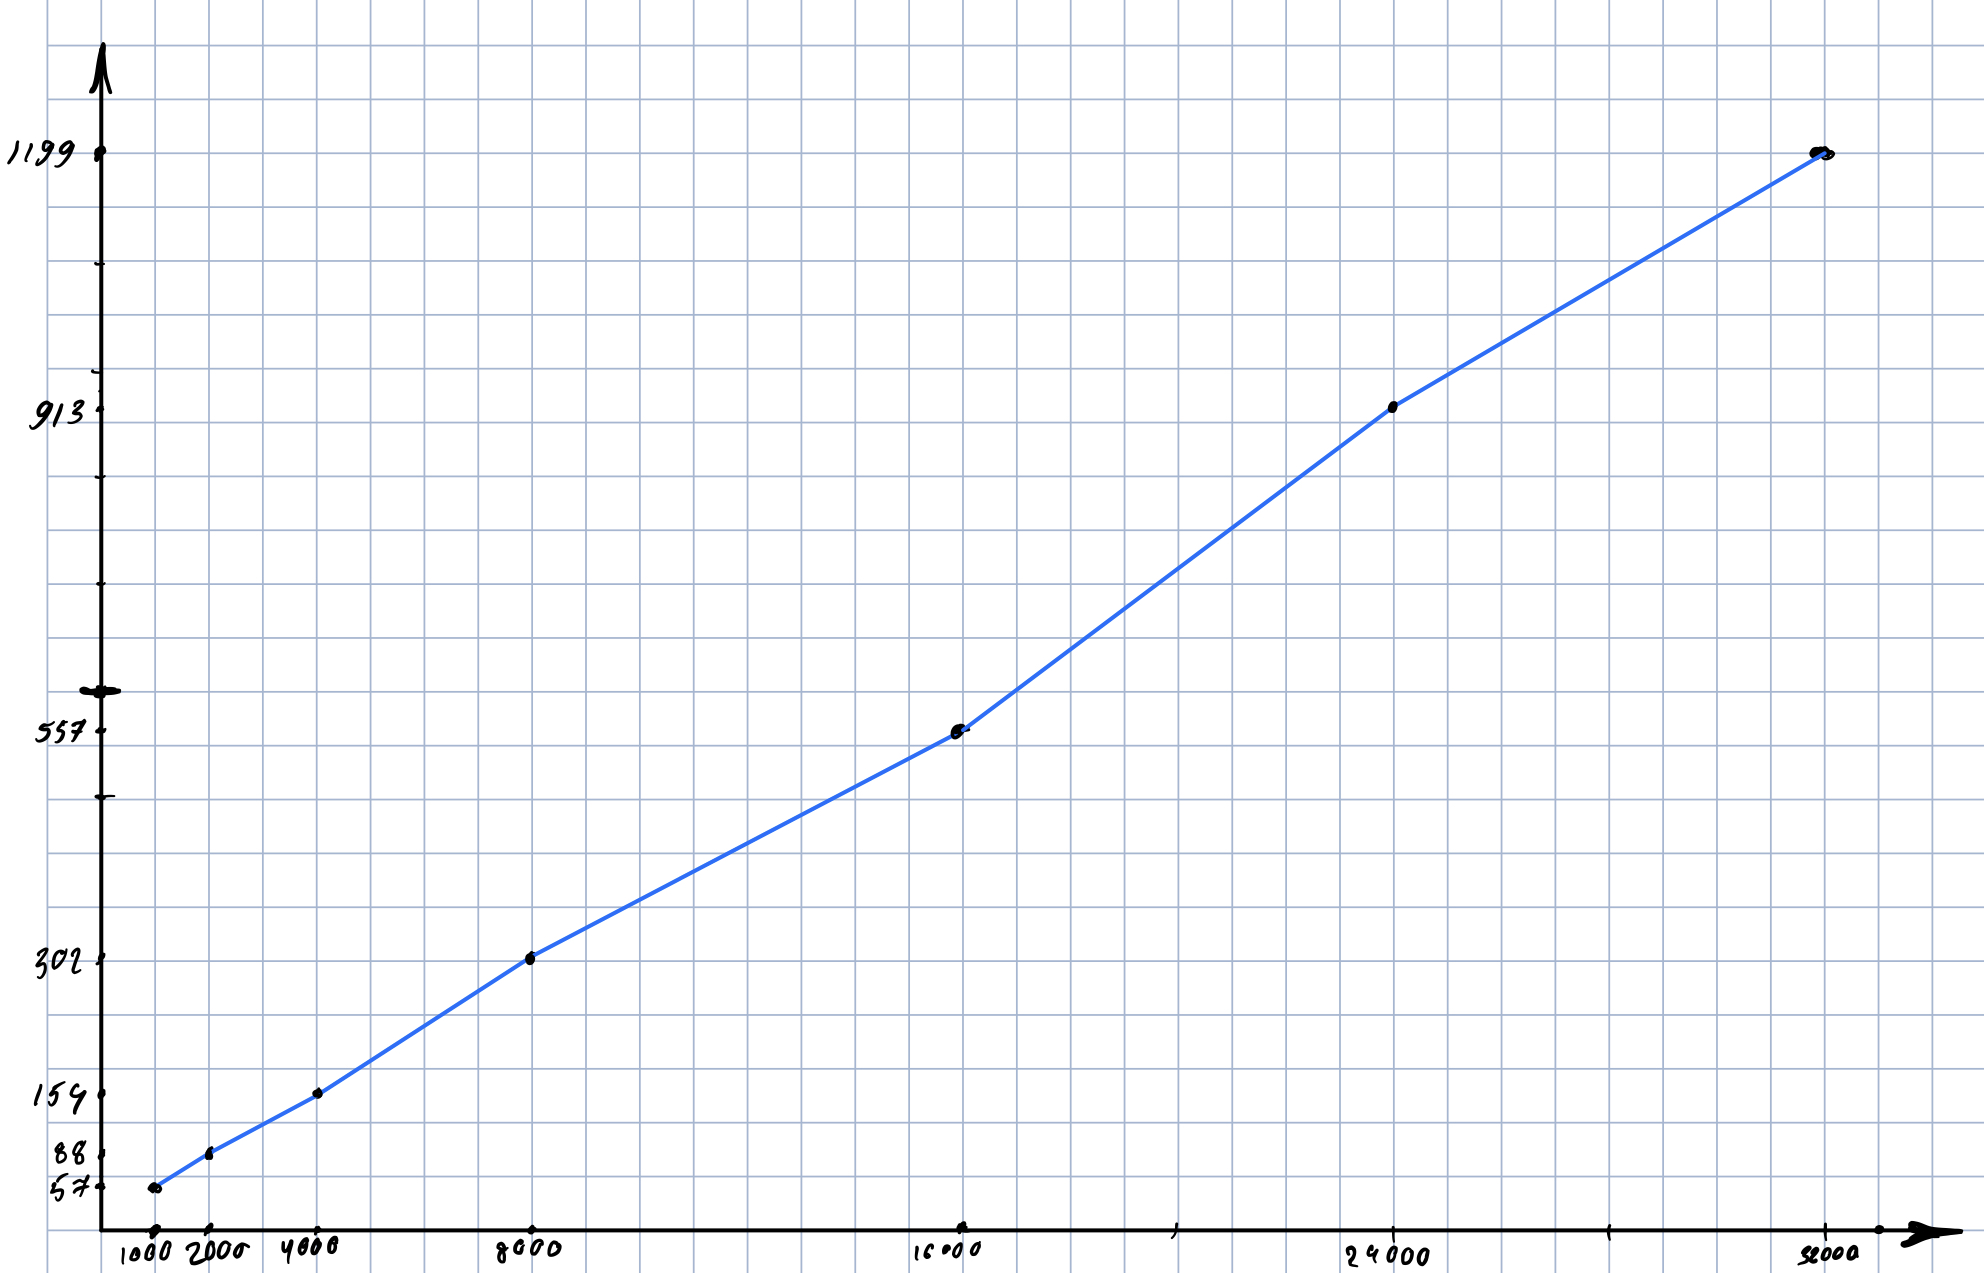
\includegraphics[width=\linewidth]{Graph}

Я действительно получаю линейное время выполнения алгоритма. Также хочу заметить, что «линейность» возрастает с количеством вхождений, так как при очень маленьком числе значений большую роль играет, так сказать, второстепенные операции, которые при большом количестве вхождением  пренебрежимо малы (линия графика не уходит в ноль).

\subsection*{Выводы}

Из данной лабораторной работы я вынес, что не обязательно всегда использовать в точности алгоритм, как он был рассказан или придуман изначально, а лучше, где это необходимо, немного модифицировать алгоритм под ту задачу, которую ты решаешь. К примеру я использовал сортировку подсчетом сразу на массиве чаров, что, по моему мнению, улучшило читаемость кода и сократило необязательные проблемы.

\end{document}

